%% Author_tex.tex
%% V1.0
%% 2012/13/12
%% developed by Techset
%%
%% This file describes the coding for rsproca.cls

\documentclass[]{rsos}%%%%where rsos is the template name


\usepackage[T1]{fontenc}
\usepackage[utf8]{inputenc}


% tightlist command for lists without linebreak
\providecommand{\tightlist}{%
  \setlength{\itemsep}{0pt}\setlength{\parskip}{0pt}}

% From pandoc table feature
\usepackage{longtable,booktabs,array}
\usepackage{calc} % for calculating minipage widths
% Correct order of tables after \paragraph or \subparagraph
\usepackage{etoolbox}
\makeatletter
\patchcmd\longtable{\par}{\if@noskipsec\mbox{}\fi\par}{}{}
\makeatother
% Allow footnotes in longtable head/foot
\IfFileExists{footnotehyper.sty}{\usepackage{footnotehyper}}{\usepackage{footnote}}
\makesavenoteenv{longtable}


\usepackage{float}

%%%% *** Do not adjust lengths that control margins, column widths, etc. ***

%%%%%%%%%%% Defining Enunciations  %%%%%%%%%%%
\newtheorem{theorem}{\bf Theorem}[section]
\newtheorem{condition}{\bf Condition}[section]
\newtheorem{corollary}{\bf Corollary}[section]
%%%%%%%%%%%%%%%%%%%%%%%%%%%%%%%%%%%%%%%%%%%%%%%

\begin{document}


%%%% Article title to be placed here
\title{Supplementary Material - A systematic machine learning approach to assess biases in population data from mobile phone applications}

\author{
Carmen Cabrera$^{1}$,
Francisco Rowe$^{1}$}

\address{
  $^{1}$Geographic Data Science Lab, Department of Geography and Planning, University of Liverpool, Liverpool, United Kingdom.\\
  $^{}$}
%%%% Subject entries to be placed here %%%%
\subject{
Mobile phone data,
Human mobility,
Explainable AI,
Spatial analysis}

%%%% Keyword entries to be placed here %%%%
\keywords{
Mobile phone data,
Human mobility,
Digital trace data,
Population estimates,
Coverage bias,
Data representativeness,
Location,
Explainable AI,
Machine learning,
Spatial bias}

%%%% Insert corresponding author and its email address}
\corres{
  Carmen Cabrera, Francisco Rowe\\
  e-mail: \href{mailto:c.cabrera@liverpool.ac.uk}{\nolinkurl{c.cabrera@liverpool.ac.uk}}; \href{mailto:fcorowe@liverpool.ac.uk}{\nolinkurl{fcorowe@liverpool.ac.uk}}
}

%%%% Abstract text to be placed here %%%%%%%%%%%%
\begin{abstract}
Traditional sources of population data, such as censuses and surveys, are costly, infrequent, and often unavailable in crisis-affected regions. Mobile phone application data (MPD) offer near--real-time, high-resolution insights into population distribution, but their utility is undermined by unequal access to digital technologies, creating biases that threaten representativeness. Despite recognition of these issues, no standard framework exists to address such biases, limiting the reliability of MPD for research and policy. We develop and implement a systematic, replicable framework to quantify and explain population coverage bias in aggregated mobile phone application data without requiring individual-level attributes. The approach combines an indicator of population coverage bias with explainable machine learning to identify contextual drivers of spatial variation in bias. Using four datasets for the United Kingdom benchmarked against the 2021 census, we show that MPD achieve higher population coverage than national surveys, but biases persist across sources and subnational areas. Population coverage bias is strongly associated with demographic, socioeconomic, and geographic features, often in complex nonlinear ways. Contrary to common assumptions, multi-application datasets do not necessarily reduce bias compared to single-app sources. Our findings establish a foundation for bias assessment standards in MPD, offering practical tools for researchers, statistical agencies, and policymakers.
\end{abstract}
%%%%%%%%%%%%%%%%%%%%%%%%%%%

\providecommand{\EndFirstPage}{%
}

\maketitle

\newpage

\section{Alternative data aggregation approaches for Facebook data}\label{alternative-data-aggregation-approaches-for-facebook-data}

Facebook Population data was aggregated temporally by averaging daily
population counts over a month and then spatially, by aggregating it
into Local Authority Districts (LADs), ensuring alignment with official
census data. To test the robustness of the population coverage bias
indicator (Equation 3.2 in the main text) under data aggregation strategies, we compared results from this
chosen approach with alternative ones. To this end, we examined
the relationship between the LAD-level bias indicator obtained from
Facebook data according to the chosen approach and from alternative
aggregation approaches. We expect to find strong linear correlations if
the bias indicator is robust to the aggregation approach. The robustness
test is shown in Figure \ref{fig:sensitivity}, where the x-axis shows
the bias indicators under the chosen method, while the y-axis shows
alternative aggregation approaches by: A) grouping into LADs, then
averaging over a month; B) averaging over a week from March 2021, then
grouping into LADs; C) grouping into LADs, then averaging over a week.
For completeness we also compare bias indicators derived from Facebook
under the chosen aggregation approach and bias indicators derived from
other data sources: D) Twitter/X, E) Multi-app 1, F) Mult-app 2.

Strong linear relationships are observed between Facebook bias
indicators across all aggregation approaches, with Pearson correlation
coefficients of 1, confirming robustness to aggregation choices. In
contrast, comparisons with other data sources show no such correlation,
indicating that different LADs exhibit larger biases depending on the
data source.

\begin{figure}[h]\label{fig:sensitivity}
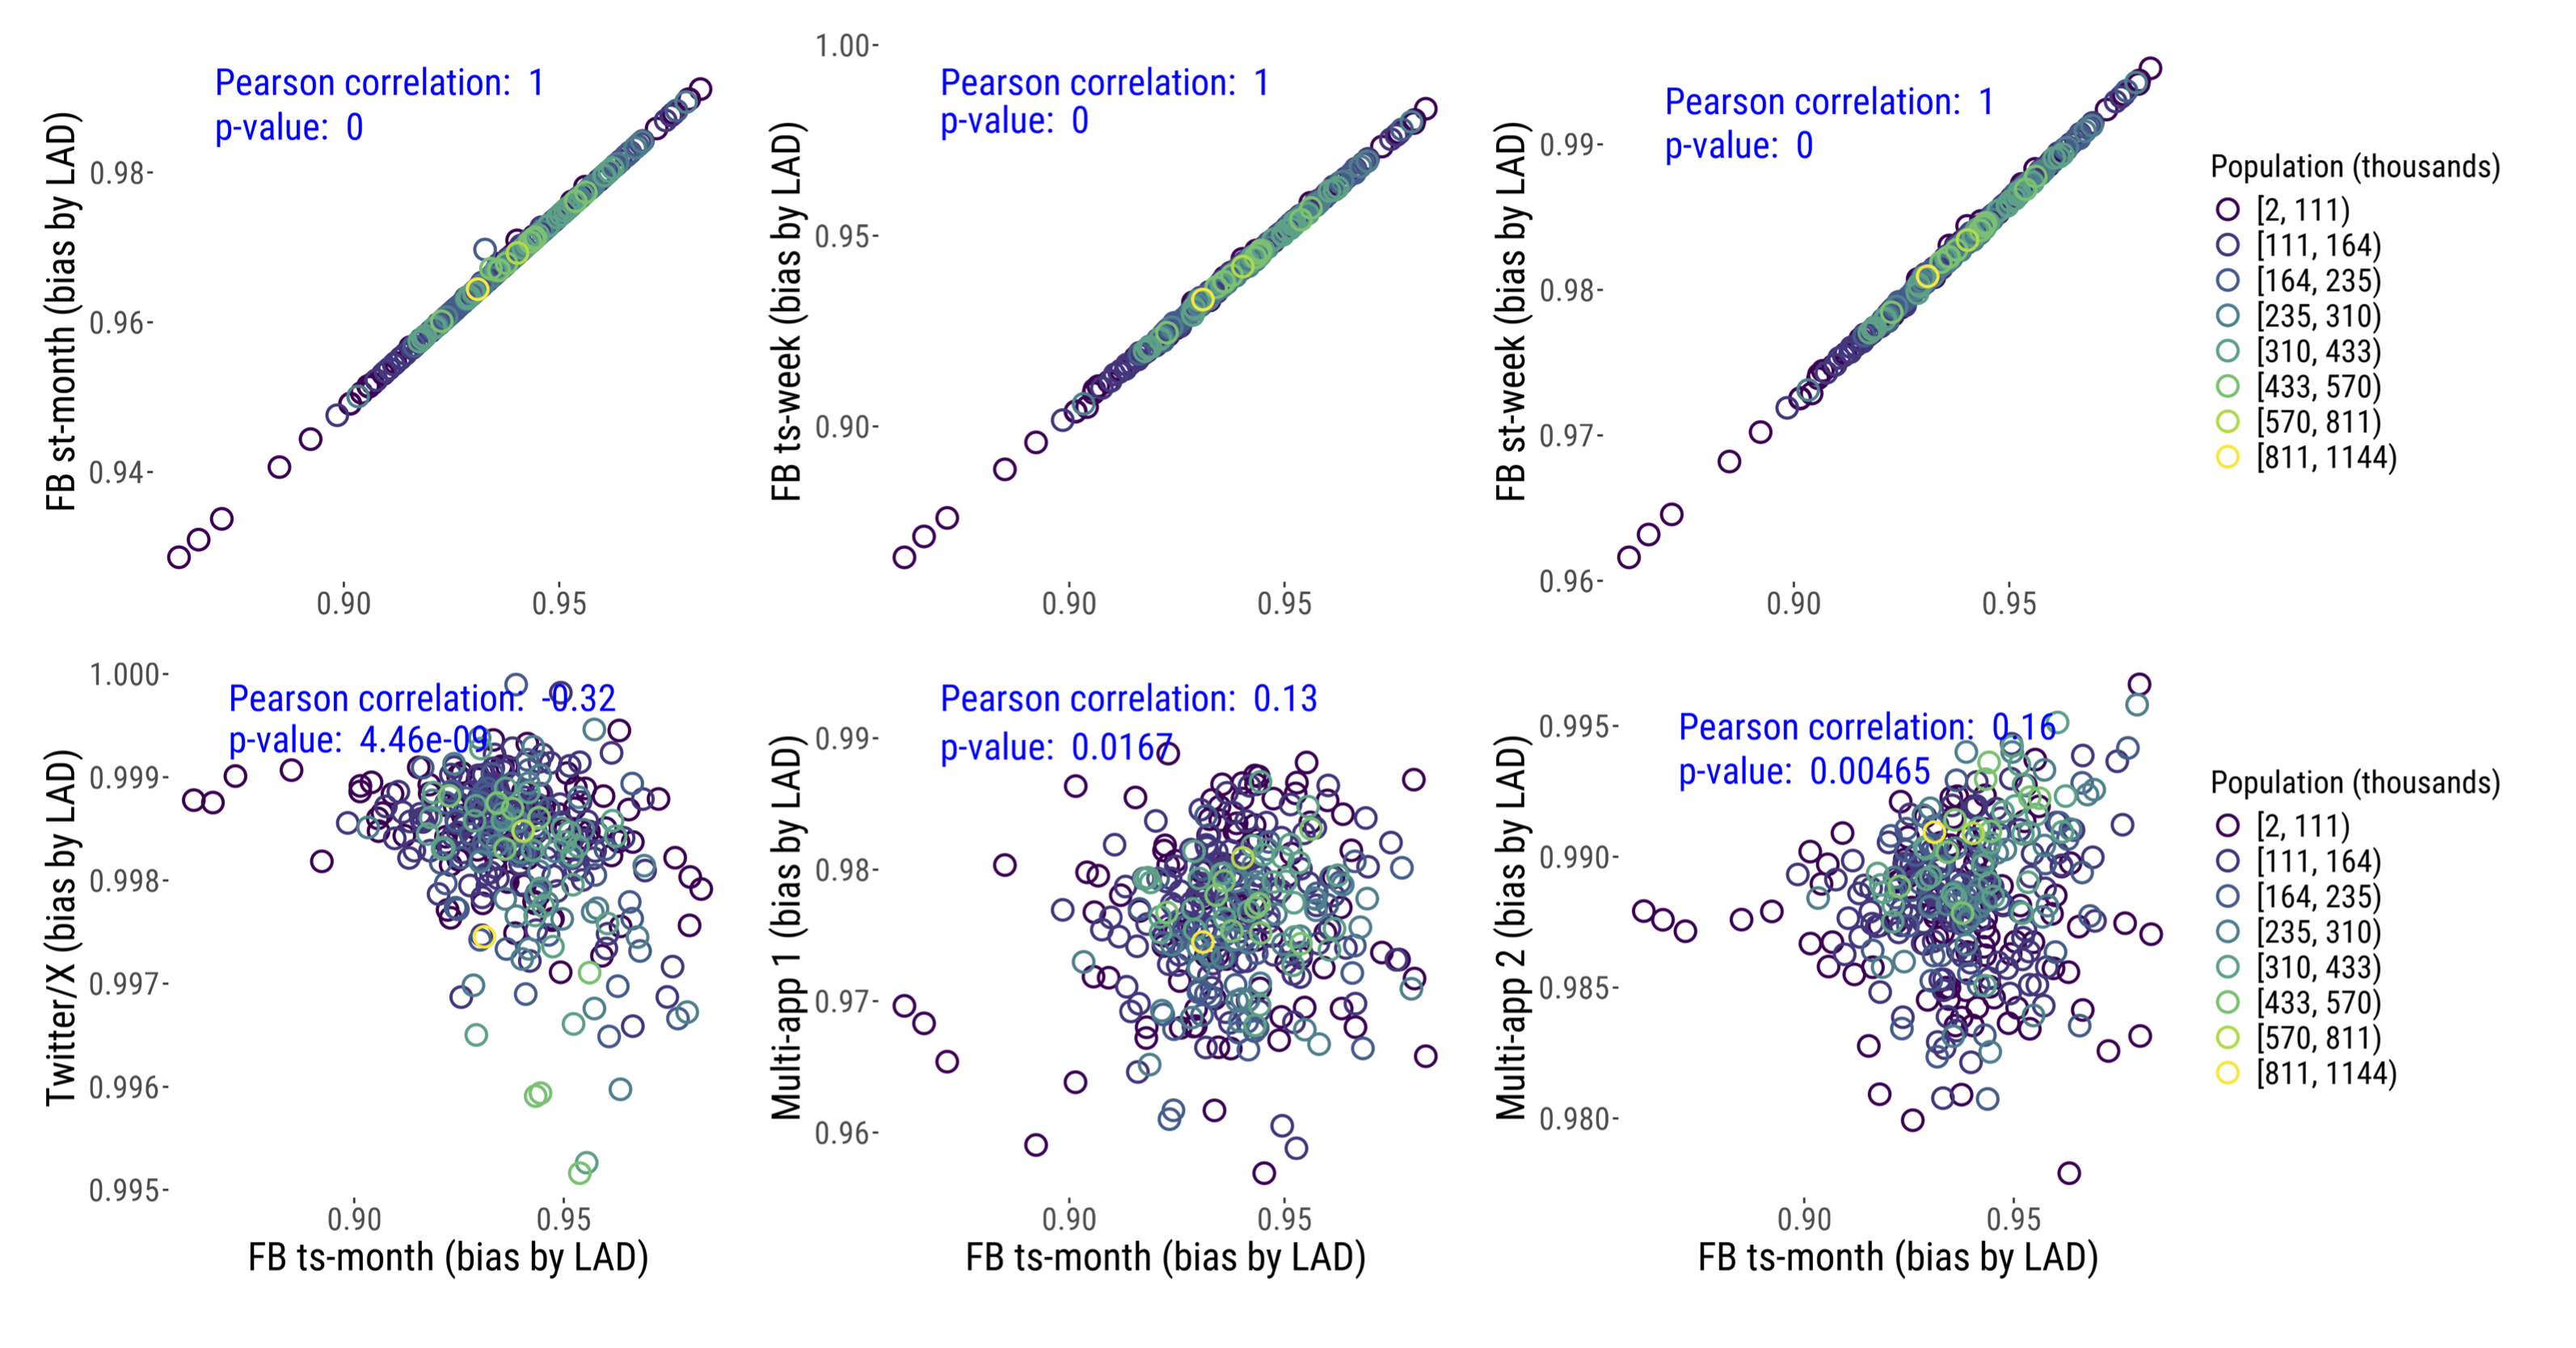
\includegraphics[width=\textwidth]{figures/Fig-compare-bias-size.png}
\caption{Robustness test of population coverage bias indicators derived from Facebook data, under alternative data aggregation approaches.}
\end{figure}

\newpage

\section{Testing for spatial autocorrelation in population coverage bias}\label{testing-for-spatial-autocorrelation-in-population-coverage-bias}

We analysed the spatial distribution of the population coverage bias indicator across LADs. Figure 3 in the main text reports Moran's I values computed using queen contiguity neighbourhoods. For comparison, Table \ref{fig:table-neighbour} presents Moran's I values and associated p-values obtained under alternative spatial weighting schemes.

\begin{figure}[h]
\label{fig:table-neighbour}
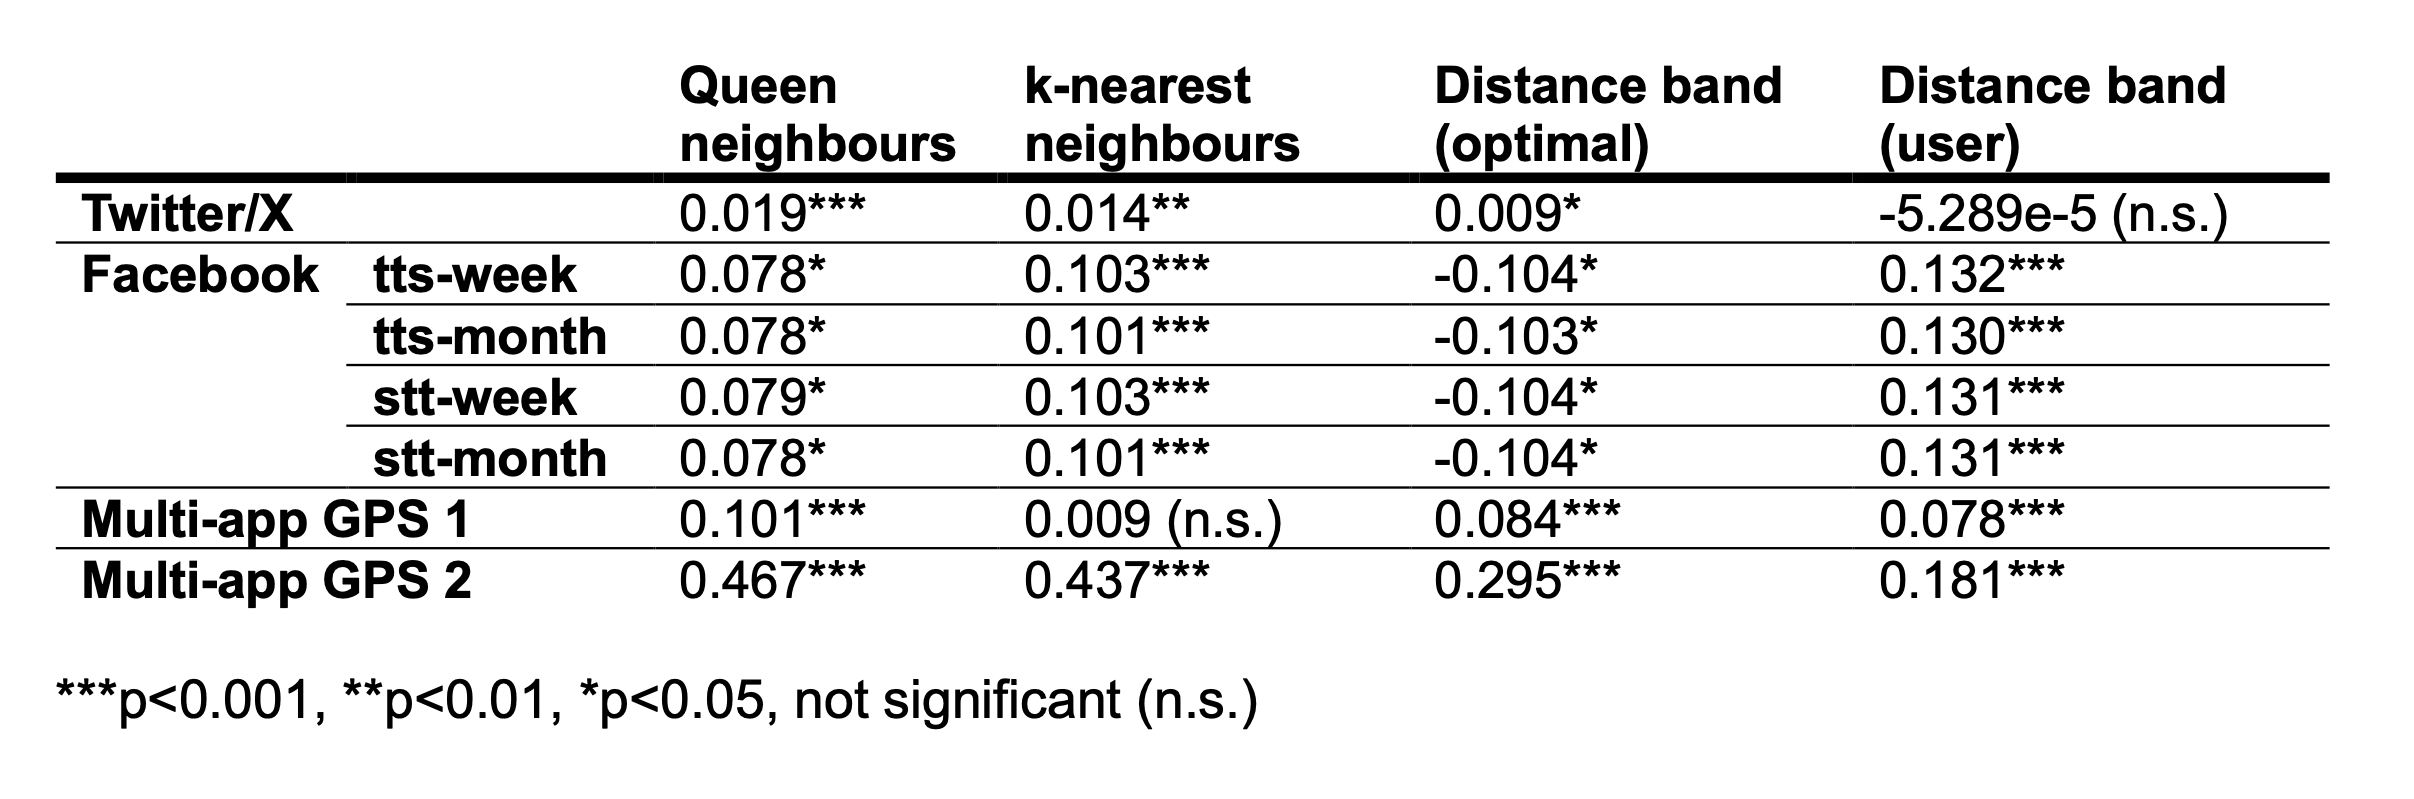
\includegraphics[width=\textwidth]{figures/Table-si.png}
\caption{Moran's I coefficients and significance,
computed according to four spatial weights schemes, 1) queen
neighbourhood, 2) k-nearest neighbours, 3) optimal distance band, and 4)
user-defined distance band.}
\end{figure}

\newpage

\ethics{This research was conducted in accordance with the ethical standards of the University of Liverpool. All data used were anonymised and analysed at an aggregate level. No identifiable personal data were accessed or processed by the authors.}

\dataccess{Please see data accessibility in the Data section. Code is openly available at \url{https://github.com/de-bias/bias-detection}.}

\aucontribute{Both authors contributed equally.}

\competing{The authors declare that they have no conflicts of interest relevant to this work.}

\funding{This work was supported by the Economic and Social Research Council (ESRC) through Smart Data Research UK programme {[}Project reference: ES/Y010787/1{]}.}

\disclaimer{Please provide disclaimer text here.}

\ack{The authors acknowledge the support of UK ESRC and of project partners: the International Organization for Migration (IOM), Meta Platforms, Inc., and Prof.~Esteban Moro.}

\bibliographystyle{RS}
\bibliography{sample.bib}


\end{document}
